\documentclass{article}
\usepackage{blindtext}
%\usepackage[utf8]{inputenc}
%\usepackage[a4paper, total={6in, 8in}]{geometry}
\usepackage{geometry}

 \geometry{
 a4paper,
 total={170mm,257mm},
 left=20mm,
 top=20mm,
 }
\usepackage{listings}
\usepackage{graphicx}


\title{ECS 132 Term Project}
\author{Alice Ma, Nicholas Jahja, Kangbo Lu, Hanzhi Ding}
\date{\today}
\begin{document}
\maketitle


\section{Problem A}
We are given student's quiz average data from three of Professor Matloff's undergraduate courses,ECS 132, 145 and 158. From this data we can also see the major of the student and the time the course was taken. From this data, we need to create a data frame and do statistical analysis on the course grades. 
    \subsection{Gathering data}
        We used R's $read.table()$ function to read the given .txt quiz data. When first looking at the returned data frame, the data has only two columns which represent the student major and quiz average. Therefore, we binded the given quarter for the quiz to the left of the student major column in the data frame by using $cbind()$ function. After binding the "year offered" column, we gave the data frame column names using $names()$ function.\\ \\
        We did this for each course's quizzes. Then we used $rbind()$ to bind one course's quizzes' data frames together and then gave it the "course name" column by using $cbind()$ function again.
        After each course's quizzes' data frame are binded together, we binded ECS132, ECS145, and ECS158 data frames together to form a data frame called ``${student\_quiz}$". The $``student\_quiz"$ data frame represents students' quiz grade of ECS 132, ECS 145, and ECS 158 courses. After using $colnames()$ function, the big combined data frame has the columns named ``course name", ``year offered" ``major", ``quiz average".
        
        \subsection{Confidence Intervals}
        \begin{itemize}
        
        \item Assuming no time trend, find approximate 95\% confidence intervals for the population mean quiz average for each of the three courses.
        \\ \\We created 3 separate data frames, one for each course (ECS132, ECS145, and ECS158), before we binded all 3 together to create one big data frame. We can go back and make use of these 3 smaller data frames to find the approximate 95\% confidence intervals for the population mean quiz average for each of the three courses by using (13.4) from the textbook:
       $$(\overline{W} - 1.96 \frac{s}{\sqrt{n}} , \overline{W} + 1.96 \frac{s}{\sqrt{n}})
       $$
       where $\overline{W}$ is sample mean, $s^2$ is sample variance, and n is sample size.
        \\\\To go into more detail:
            \begin{itemize}
                \item The sample mean quiz averages for each of the 3 data frames can be found be accessing the "quiz average" column of each data frame, putting each of them into the form of a vector, and using that vector as a parameter for the mean() function.
                
                \item Similarly, the sample variance quiz averages can be found using the same "quiz average" vector from each of the 3 course data frames. Using the mailing tube for variance, $Var(X) = E(X^2) - (EX)^2$, we simply square the "quiz average" vector of each course data frame, take the mean of those values, and subtract them by their respective sample means which we all calculated just before this. Taking the square root of the sample variances will give us the sample standard deviations. 
                
                \item To find standard error for each course we divide their respective standard deviations, s, by the square root of their respective sample sizes, n, $\frac{s}{\sqrt{n}}$. Then, multiply the standard errors by 1.96 to obtain the radius for each course, and finally subtract and add the radius by each course's sample mean quiz average to obtain the 95\% confidence interval for the population mean quiz average for each of the three courses. 
           \end{itemize}
           The 95\% confidence interval for the population mean quiz average for each of the three courses come out to be the following:\\
            
            ECS 132: (2.542122, 2.758809)
            
            ECS 145: (2.529258, 3.403172)
            
            ECS 158: (3.099078, 3.31404)
\item Assuming no time trend, find an approximate 95\% confidence interval for the difference in population mean quiz averages for ECS 132 and 145.
\\\\Obtaining the confidence interval for the difference in population mean is quite similar to our previous problem. The biggest difference is our new calculation for standard error of the difference in sample mean. We apply (13.21) from the textbook to find the confidence interval, 
            $$(\overline{W} - \overline{Y} - 1.96 \sqrt{\frac{s_1^2}{n_1} + \frac{s_2^2}{n_2}}, \overline{W} - \overline{Y} + 1.96 \sqrt{\frac{s_1^2}{n_1} + \frac{s_2^2}{n_2}})$$ \\
            where $\overline{W}$ is sample mean quiz average of ECS132, $\overline{Y}$ is sample mean quiz average of ECS145, $s_1^2$ is sample variance quiz average of ECS132, and $s_2^2$ is sample variance quiz average for ECS145. All of these values from (13.21) were already found and saved as variables from the calculations we did to solve the previous problem where we found each course's respective 95\% confidence interval for population mean quiz average. \\
            
            The 95\% confidence interval for the difference in population mean quiz averages for ECS132 and ECS145 come out to be: (-0.8279351, -0.4350624)

        
\item Assuming no time trend, find an approximate 95\% confidence interval for the difference in population mean quiz averages in ECS 145 between the two majors.
\\\\ Similar to the previous problem, we need to find the difference in two population mean quiz averages. The big diffrrence between this problem and the previous problem is that population mean quiz averages are between two majors in the same class, instead of two courses. So we still apply (13.21) from the textbook to find the confidence interval,
            $$(\overline{W} - \overline{Y} - 1.96 \sqrt{\frac{s_1^2}{n_1} + \frac{s_2^2}{n_2}}, \overline{W} - \overline{Y} + 1.96 \sqrt{\frac{s_1^2}{n_1} + \frac{s_2^2}{n_2}})$$
            where $\overline{W}$ is sample mean quiz average of CS major, $\overline{Y}$ is sample mean quiz average of CSE major, $s_1^2$ is sample variance quiz average of CS major, and $s_2^2$ is sample variance quiz average for CSE major. We get sample mean quiz averages using $subset()$ and $mean()$ functions.\\
            
            All of these values from (13.21) were already found and saved as variables from the calculations we did to solve the previous problem where we found each course's respective 95\% confidence interval for population mean quiz average. \\
            
            The 95\% confidence interval for the difference in population mean quiz averages in ECS 145 between the two majors come out to be: (-0.266078, 0.1619864)

    \end{itemize}
        \subsection{Establishing Trends with a Linear Regression Model}
        \item Fit a linear regression model in which quiz average is predicted from year, course and major. For the last two, create dummy variables (Sec. 21.12). Use this to determine whether there is a substantial time trend. Also use it to compare ECS 132 and 145, and CS majors to CSE. (This is different from above, because now we are adjusting for a possible time trend.)
        
            \begin{itemize}
                \item We must first create dummy variables for the "major" and "course name" columns of our data frame. 
\\\\Since there are only two majors, CS and CSE, only one dummy variable is needed for majors. From the data frame, the CSE major factor value was default set to 1, and the CS major factor value was set to 2. Taking advantage of this fact, we can play with the data frame "major" column and create a vector called "is\_cs\_major" equal to the size of the sample size and have it contain only the values 0 and 1, where 0 corresponds to a student majoring in CSE and 1 corresponds to a student majoring in CS. In this way we have an indicator variable for students who are CS majors. 
                    
 \\With 3 courses in our data frame, we need to create 2 dummy variables. Similar to how we created our first dummy variable, we have two indicator variables, one for ECS145 and one for ECS158. The default values for ECS132, ECS145, and ECS158 were 1, 2, and 3 respectively. We use this information to create our vectors, "is\_ECS145" and "is\_ECS158" which correspond to the ECS145 and ECS158 indicator variables. If both indicator variables are 0 for a given student, that that student must be in ECS132.

                
                \item With the dummy variables created, we simply make the call to the summary() and lm() functions to obtain information on our coefficients:
                
\lstset{breaklines=true}
\begin{lstlisting}[math escape]
summary(lm(student_quiz$`quiz average' ~ student_quiz$`year offered'+ is_cs_major+ is_ECS145 + is_ECS158))
\end{lstlisting}

                where student\_quiz is the name of our data frame.
                With this information, we can answer the current problem:
                
                \begin{description}
                    \item[Is there a substantial time trend?] :
                    
                    \\The coefficient for ``year offered" is 0.01925 with a standard error of 0.02291. Subtracting and adding 1.96 multiplied by the standard error from the coefficient will provide us with the 95\% confidence interval of the change in population mean quiz average over change in time, with the unit of time being years. \\
                    The confidence interval comes out to: (-0.0256536, 0.0641536) \\
                    This means that for every year passed, we are 95\% confident that the population mean quiz average changes by some value within this interval. As we know, the quiz scores are within the interval [0,4]. The 95\% confidence interval has relatively small values. In addition, the confidence interval contains 0, meaning that the quiz average for a given year can either decrease or increase. Given this information, we have determined that there is not a substantial time trend. \\
                    Alternatively, a significance test can be done, checking the given t-value for the ``year offered" coefficient: 0.840. We can see that this value is $(-1.96 < 0.840 < 1.96)$, meaning that the factor of time is not significant. 
                    
                    \item [Compare ECS132 and ECS145 (adjusting for possible time trend)]: \\
                    The coefficient for ``is\_ECS145" is 0.66235 with a standard error of 0.09029. Since we created dummy variables for ECS145 and ECS158, if both indicator variables are 0, the it is given that the student is from ECS132. Therefore, the ``is\_ECS145" coefficient gives the difference in sample mean quiz averages of ECS145 and ECS132. Subtracting and adding 1.96 multiplied by the standard error from the coefficient will provide us with the 95\% confidence interval of the difference in population mean quiz average for ECS145 and ECS132. \\
                    The confidence interval comes out to : (0.4853816, 0.8393184)\\
                    On average, students from ECS145 score between 0.4853816 to 0.8393184 higher on quizzes than students from ECS132.
                    
                    \item [Compare CS and CSE majors (adjusting for possible time trend)] : \\
                    The coefficient for ``is\_cs\_major" is -0.11987 with a standard error of 0.07395. Subtracting and adding 1.96 multiplied by the standard error from the coefficient will provide us with the 95\% confidence interval of the difference in population mean quiz averages between the two majors. \\
                    The confidence interval comes out to : (-0.264812, 0.025072)\\
                    On average, CS students score between -0.264812 to 0.025072 difference in quiz scores than CSE students.

                \end{description}
                


        \item Do an analysis of your choice that investigates whether there is a time trend in the proportion of CS majors in our department, based on this data.
\\\\Using the dummy variable ``is\_cs\_major" we created from the previous problem and the "year offered" column of our "student\_quiz" data frame, we can fit a linear regression model in which proportion of CS majors is predicted from year. The "is\_cs\_major" works to find proportion of CS majors because it is a vector of size equal to sample size and contains values 0 and 1, with 0 corresponding to a student not majoring in CS (in this case, the only two majors in our data set are CS and CSE, so any student that is not in CS automatically means he/she is in CSE), and 1 corresponding to a student majoring in CS. Taking the mean of this vector will therefore give us the sample proportion of CS majors. We make the call to summary() and lm() to obtain information on our coefficients: \lstset{breaklines=true}
\begin{lstlisting}[math escape]
summary(lm((is_cs_major ~ student_quiz$`year offered')) 
\end{lstlisting}
           
            
            The coefficient for ``year offered" is 0.04941 with a standard error 0.01409. Subtracting and adding 1.96 multiplied by the standard error from the coefficient will provide us with the 95\% confidence interval of the change in population proportion of CS majors (by population in this case we mean in our department) over the change in time, with the unit of time being years. \\
            The confidence interval comes out to: (0.0217936, 0.0770264) \\
            This means that the population proportion of CS majors increases by a value between the interval (0.0217936, 0.0770264) per year. With the given t-value of 3.506, and since 1.96 $<$ 3.506, we can conclude that there is a substantial time trend in the proportion of CS majors in our department.



    \end{itemize}
    
\section{Problem B}
    \subsection{Collecting and Organizing Data}
    By sending a GET request to the official exam page for each course, we can obtain the HTML files that contains  the link to each exam file by matching the pattern "(?<=(href=$\textbackslash$"))(.)*.tex(?=$\textbackslash$")" with calling str$\textunderscore$extract$\textunderscore$all() function. Then, we used read the file using readLines() function.
    \\\\
    After reading the .tex files from the server, we used regular expression "([\{]?)[$\textbackslash\textbackslash$](.)*[\}]" to filter out the latex expression in the begining of each line. Then, we used "tm" package's functions to clean create corpus, a collection of text file for analysis.\\
    By using the "tm\_map()" function from "tm" package, we are able to clean the data through converting words to lower cases, removing punctuation, removing numbers, taking away white spaces in the corpus, and removing our specified stop words.
    \\\\
    We also split our data, choosing 50 files from our total 265 files for testing data, and saving the remaining 215 files to use as training data. We determined the files to remove from each course by proportion to the total number of files that were available to choose from. For example, ECS 50 had a total of 62 files, so we choose 13 files to remove as testing data compared to choosing one file as test data from ECS 154B that only had 3 files total. 
    
    \subsection{Choosing Predictor Variables}
    To help us understand the data, and also for fun, we decided to generate a word cloud to better visualize our training data. Below is an example of ECS 132's word cloud:
        \begin{wrapfigure}
        \centering
        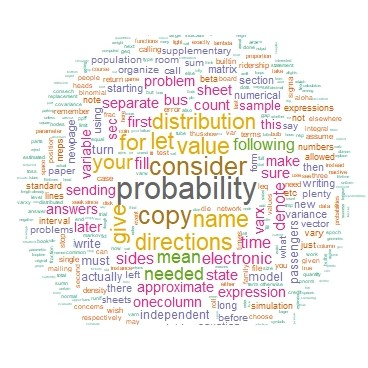
\includegraphics[scale=1]{ECS132.jpeg}\\
        \end{wrapfigure}
    
    To create document term matrices we first wrote a ``create\_dtf\_matrix()" function. In this function, we used the ``DocumentTermMatrix()" function to create a dtf with cleaned data and count the frequency by ``colSums()" and then ordered it in decreasing order. After all, we used ``create\_dtf\_matrix()" to to create the document term matrices for each course.
        \\\\
        After examining the frequency of the words for all nine courses generated by the Document Term Matrix, we decided to take the two words that appeared most often in quizzes for each course. We decided to choose two words per course because we wanted to stay close to 14 predictor variables. We had a total of 265 total files, from these files we allocated 50 files as test data and kept 215 files as training data. $\sqrt{215} \approx 14.6$ With nine courses and two predictor variables for each, that comes out to 18 predictor variables, however the predictor variable `time' was overlapped between two courses. To mitigate this issue, we simply removed this extra column. Limiting the number of predictor variables was important to keep our accuracy high as too many predictor variables can cause our accuracy to decrease due to redundant predictors. 
    
    \subsection{Fitting our Model}
        \begin{description}
        \item[Creating indicator variables for all 9 courses]:\\
        When we obtained our training data, we organized them in order of course name, so the first 49 rows of the training data matrix were exams from ECS 50, the next 66 rows were exams from ECS 132, and so on. The number of exams in each course used for training data were already determined when we split the data into training and testing sets. This makes it easy for us to create vectors for indicator variables for each of the 9 courses. Each vector has total size of 215, which matches the size of the training data, and we first set all values to 0. Then since the training data is already sorted by course name, we can update the indices of each indicator variable vector accordingly. For example, since we know only the first 49 rows of the data are exams from ECS50, we update the ``is\_ECS50" vector so that the first 49 are set to 1, and the rest of the values remain at zero. Continuing on, we know the next 66 rows of the data are all the exams from ECS132, so we update the ``is\_ECS132" vector where the first 49 values remain as zero, the next 66 values are set to 1, and the rest of the values remain as zero. We continue this process to create all 9 indicator variables for the 9 courses. 
        \item [Create the model]: \\
        With the indicator variables and the training data matrix already created, we simply call the glm() function 9 separate times. For example, with ECS 50 we call the function : \\
        glm(is\_ECS50 $\sim$ dtf, family = binomial), \\
        where is\_ECS50 is the indicator variable vector for ECS 50, and dtf is the name of our training data matrix. We repeat this function call 9 times, changing only the indicator variable used. This provides us with the 9 logit models and the coefficients necessary to calculate the probabilities for a given exam to be in each of the 9 courses.
        
        \item [Test the model]:\\
        Using the mailing tube (16.2) for logistic function in Chapter 16, we are able to evaluate probability and predict which course the test exam is. We first stored the coefficients of 9 generalized linear models into a list. The list now contains the coefficients for each model. And then, we multiplied each term of the coefficients with the formatted test exam column value together to obtain the $u$ for the logistic function. With the value of $u$ found, we can use (16.2) to find each of the 9 course probabilities, corresponding to each of the 9 logit models. Then, since we know the actual course for each exam in the testing set, we simply choose the highest course probability for each testing set exam, and see if the predicted course matches with the true course. After going through all 50 cases in our testing set, we obtain the calculated prediction accuracy of 72\%
        
        \end{description}
\section{Team Member Contribution}
     All group members have been actively contributed to the term project. We spent time together to figure the problems out. Kangbo Lu gathered, cleaned, tidied data and tested models. Hanzhi Ding and Kangbo analyzed Confidence Interval for couple parts in Problem A. Alice Ma and Nicholas Jahja analyzed for Confidence Intervals for the other parts and predictive models. Hanzhi visualized word frequency for Problem B to help select the stop words. Everyone wrote the Latex together after finishing coding, and Alice formatted it.

\end{document}
